\documentclass{l4proj}

\usepackage{url}
\usepackage{fancyvrb}
\usepackage[final]{pdfpages}
\usepackage[acronym,toc]{glossaries}
\usepackage{listings}
\usepackage{textcomp}

\newcommand{\tex}{\TeX}
\newcommand{\BibTeX}{B{\sc ib}\TeX}
\newcommand{\bibtex}{\BibTeX}
\newcommand{\latex}{\LaTeX{} }
\newcommand{\revisit}{\#\#\#}
\newcommand{\cs}{C\#}
\newcommand{\naive}{na\"{\i}ve}
\makeindex
\makeglossaries

%						Short plural key				 Long plural key
\newacronym[\glsshortpluralkey=smpls,\glslongpluralkey=samples]{smpl}
%key		 value
{SAMPLE}{Sample entry}

\newglossaryentry{sample}{name={sample}, description={a sample glossary entry}}
% ==========================================
% 	Acronyms 				acm
% 				  key  		displayed		Full string
\newacronym{acm}		{ACM}				{Association for Computing Machinery}
\newacronym{ajax}		{AJAX}			{Asynchronous JavaScript And XML}
\newacronym{aod}		{AOD}				{Architecture Overview Diagram}
\newacronym{asp}		{ASP}				{Active Server Pages}
\newacronym{bat}		{.BAT}				{Batch File}
\newacronym{case}		{CASE}			{Computer-Aided Software Engineering}
\newacronym{ci}			{CI}				{Continuous Integration}
\newacronym{clr}		{CLR}				{Common Language Runtime}
\newacronym{css}		{CSS}				{Cascading Style Sheet}
\newacronym{fnh}		{FNH}				{Fluent NHibernate}
\newacronym{html}		{HTML}			{HyperText Markup Language}
\newacronym{http}		{HTTP}			{HyperText Transfer Protocol}
\newacronym{id}			{ID}				{Identifier}
\newacronym{ide}		{IDE}				{Integrated Development Environment}
\newacronym{jre}		{JRE}				{Java Runtime Environment}
\newacronym{js}			{JS}				{JavaScript}
\newacronym{json}		{JSON}			{JavaScript Object Notation}
\newacronym{jvm}		{JVM}				{Java Virtual Machine}
\newacronym{linq}		{LINQ}			{Language Integrated Query}
\newacronym{msdnaa}	{MSDNAA}		{Microsoft Developer Network Academic Alliance}
\newacronym{msss}		{MSSQL}			{Microsoft SQL Server}
\newacronym{msvs}		{MSVS}			{Microsoft Visual Studio}
\newacronym{mvc}		{MVC}				{Model View Controller}
\newacronym{oo}			{OO}				{Object-Oriented}
\newacronym{sql}		{SQL}				{Structured Query Language}
\newacronym{ssh}		{SSH}				{Secure Shell}
\newacronym{svn}		{SVN}				{Subversion}
\newacronym{ui}			{UI}				{User Interface}
\newacronym{uml}		{UML}				{Unified Modelling Language}
\newacronym{uri}		{URI}				{Uniform Resource Identifier}
\newacronym{url}		{URL}				{Uniform Resource Locator}
\newacronym{xml}		{XML}				{eXtensible Markup Language}

% ==========================================
% 	Glossary terms
% 				  			key  	  Name						 									Explanation
\newglossaryentry{svntag}	{name={SVN Tag}, 									description={A snapshot of a project in time, saved with a human-readable name}}
\newglossaryentry{unix}		{name = {UNIX},										description={An open-source operating system}}
\newglossaryentry{net}		{name = {.NET},										description={An application development framework by Microsoft}}
\newglossaryentry{contInt}{name = {Continuous Integration},	description={A technique which runs all tests after each change to a solution's code repository.}}
\newglossaryentry{vm}{name = {Virtual Machine},							description={Hardware emulator: allows running of a system as if it were on its own machine where it is actually running as a process on machine}}

\lstdefinelanguage{CSharp}
{
 sensitive=true,
 morekeywords=[1]{
  select, from, where, % added for Linq support
  abstract, as, base, break, case,
  catch, checked, class, const, continue,
  default, delegate, do, else, enum,
  event, explicit, extern, false,
  finally, fixed, for, foreach, goto, if,
  implicit, in, interface, internal, is,
  lock, namespace, new, null, operator,
  out, override, params, private,
  protected, public, readonly, ref,
  return, sealed, sizeof, stackalloc,
  static, struct, switch, this, throw,
  true, try, typeof, unchecked, unsafe,
  using, virtual, volatile, while, bool,
  byte, char, decimal, double, float,
  int, lock, object, sbyte, short, string,
  uint, ulong, ushort, void},
 morecomment=[l]{//},
 morecomment=[s]{/*}{*/},
 morecomment=[l][keywordstyle4]{\#},
 morestring=[b]",
 morestring=[b]',
}
\lstset{
 backgroundcolor=\color[rgb]{0.95, 0.95, 0.95},
 tabsize=2,
 rulecolor=,
 basicstyle=\scriptsize,
 upquote=true,
 aboveskip={1.5\baselineskip},
 columns=fixed,
 showstringspaces=false,
 extendedchars=true,
 breaklines=true,
 prebreak = \raisebox{0ex}[0ex][0ex]{\ensuremath{\hookleftarrow}},
 frame=single,
 showtabs=false,
 showspaces=false,
 showstringspaces=false,
 identifierstyle=\ttfamily,
 keywordstyle=\color[rgb]{1.0,0,0},
 keywordstyle=[1]\color[rgb]{0,0,0.75},
 keywordstyle=[2]\color[rgb]{0.5,0.0,0.0},
 keywordstyle=[3]\color[rgb]{0.127,0.427,0.514},
 keywordstyle=[4]\color[rgb]{0.4,0.4,0.4},
 commentstyle=\color[rgb]{0.133,0.545,0.133},
 stringstyle=\color[rgb]{0.639,0.082,0.082},
}
% ==========================================
% ==========================================

\begin{document}
\title{\bibtex{} Entry Manager}
%\subtitle{A Software Solution for Management of \bibtex{} References}
\author{John Lewis Thow [0701068]}
\date{\today}
\maketitle

% old:
%This dissertation discusses a software solution implemented in \cs{} under the Microsoft.NET application framework to address some of the problems associated with management of \bibtex{} entries by a group of authors collaborating on a one or more pieces of work.

\begin{abstract}
Authors of \latex documents often maintain lists of bibliographic references stored in \bibtex{} format.  The management of such lists can pose several problems to authors. These are often exacerbated because multiple authors frequently have to share a set of references; for example, when they are developing a paper collaboratively.

Authors would thus value and benefit from a system of maintaining and managing \bibtex{} records that overcame these problems particularly if it enabled them to maintain and manage the records in a collaborative way. 

Two previous projects undertaken by students in the School of Computing Science at the University of Glasgow resulted in a desktop solution and a web-based solution that, overcame some of the problems; both of the studies provide the foundation on which this project is built.

The dissertation identifies some of the problems that continue to hamper the effective management of \bibtex{} entries.  It examines some of the previous attempts to resolve them, discusses the requirements that any improved solution should meet and describes how such a solution was designed and technically implemented.  The dissertation goes on to describe and discuss a set of evaluations and tests to determine the success of the software solution produced.

The author aimed to produce a usable, useful and stable software system that addressed the identified needs of collaborating authors while following disciplined software engineering methods.

The software solution produced was found to be a success �-- an outcome determined by statistical analysis of evaluation participants' responses to a questionnaire.  The measurements derived from this showed that all participants reacted positively to questions on the usability of the software solution.  Moreover, they encouraged further development of the solution and even suggested specific areas of further work.   These areas of further development, along with some areas conceived by the author and supervisor of this dissertation, are included in the discussion of future work in the conclusion section.

The fidelity of the software solution proposed was limited by the length of the academic year.  Some of the shortcomings of the solution include sub-optimal authentication during registration and over-simplification of the search engine and security protocol. These and other residual issues are discussed in the final chapter.
\end{abstract}


%\chapter*{Thanks and Acknowledgements}
\newpage
\section*{Acknowledgements}
I owe a debt of gratitude to the following individuals for the support they gave me while designing, developing and evaluating the software solution and while preparing this dissertation:
\begin{itemize}
\item Dr David Manlove of the University of Glasgow;
\item Mr Gregg O'Malley of the University of Glasgow;
\item Dr Colin Perkins of the University of Glasgow;
\item Mr Graham Mooney of Cisco Systems;
\item Mr Thomas Anderson of the Amor Group;
\item My family, friends and classmates;
\item All of the volunteers who took part in my evaluation;
\item The staff in the School (Department!) of Computing Science at the University of Glasgow, both retired and active who have had an input on my education over the past 4 years.
\end{itemize}

\educationalconsent
%
%NOTE: 	if you include the educationalconsent (above) 
% 			and your project is graded an A then
%      	it may be entered in the CS Hall of Fame

\tableofcontents
\glsresetall{}
%==========================================================
\chapter{Introduction}
\label{intro}
The introduction spells out some preliminary information and aims of the project to ensure that the reader is familiar with the area of the project and what the high-level goals of the project are.

\section{Preliminaries}
\subsection{\TeX{}}
In the words of its creator, \TeX{} is ``a [new] typesetting system intended for the creation of beautiful books---and especially for books that contain a lot of mathematics'' \cite{DK84}.  The \TeX{} program is a set of primitive commands for basic typesetting; it also allows users to create more complex commands in terms of simpler ones.  Donald Knuth created the \TeX{} program in 1978 and a subsequent version of it makes up the core of the program that is used today \cite{TeXOrigin}.  To realise the full potential of \TeX, users require considerable experience with programming techniques.  As a result, the use of \TeX{} on its own is limited to typography and programming professionals \cite{KD95}.

\subsection{\LaTeX}
To allow non-experts to exploit the most powerful features of \TeX{} without first having to familiarise themselves with programming techniques, \latex was created by Leslie Lamport in 1985. \latex contains a range of commands written in terms of primitive \TeX{} commands, providing users with a set of higher-level commands for the production of complex documents.  It also allows for a separation of concerns between the information that is being presented from the formatting that has to be applied when publishing \cite{KD95}.

It is standard to find a bibliography at the end of a scientific publication. \latex provides an `environment'\footnote{An environment is used to specify an area of a document where the text has to be presented with different indentation, line width, typeface and so on \cite{KD95}.  The environment used by \latex is called `\texttt{thebibliography}'.} which allows bibliographic references to be listed and stored in one area of a document \cite{KD95}, but this approach requires that each document has its own list of references, which may lead to redundancy and inconsistency if, for example, an author has multiple publications on the same subject. 

\subsection{\bibtex}
\bibtex{} is an auxiliary program to \latex which provides the authors with the ability to store all of their bibliographic references in one or more files.  Each reference, or `entry', is uniquely identified by its cite key, which is used within a document where the reference is made.\footnote{A reference to a citation is inserted by using the \latex command \texttt{$\backslash$cite\{citeKey\}} in the body of the document, where `citeKey' is the identifier of the reference in one of the referenced bibliographic files}

The benefit of using \bibtex{} as a means of bibliography production is that a file set is easier to maintain than having sporadic files, each with individual collections of references, as one file can be re-used for all publications.

\section{Problem Statement, Aims and Motivation}
An author is likely to amass a vast number of bibliographic references, through having to make a large number of citations over years of work.  The task of managing this library of references is an issue in itself.  For example, authors might have clashing cite keys or entries that are recorded twice in the library.  It is also crucially important to ensure that field names are not misspelled --- especially when a field is optional, as this results in it being ignored without warning \cite{OP88}.

The problem of managing entries is exacerbated when multiple users that are collaborating on a piece of work need to share collections of entries: with no management system in place, users have to find a way to consistently and unerringly distribute files by email and other manual methods, while ensuring that there have been no clashing entries.  This includes ensuring that a user can add, edit, delete, import and export their entries to and from the collection.

An anecdotal example of the \bibtex{} file management problem exists within the School of Computing Science at the University of Glasgow: the Matching group frequently collaborated on papers and maintained a single list of references, entitled \texttt{matching.bib}.  Distribution of this file was performed manually by email after changes were made to the list by any of the members of the Matching group; it was an understandably error-prone and unwieldy method of distribution of the references.

The main aim of this project is to identify a solution to solve the problems defined and described above.  The author was motivated towards this project because the problem is one that interests him and finding a solution would offer practical benefits.  Exploring the subject would also enable him to:
\begin{enumerate}
	\item Develop a good understanding of the technologies used;
	\item Observe good software engineering practice during development and testing;
	\item Develop professional attitude and strategy for dealing with project matters;
	\item Produce a user-friendly system;
	\item Ensure that the system is robust and reliable (as far as programming is concerned);
\end{enumerate}

%it will be important to evaluate both the usability and effectiveness of the product by   \bibtex{} entries for multiple users.

\section{Outline of Report}
%List these as references to each section!
This report will discuss how the author analysed problems that are commonly encountered with managing \bibtex{} references and identify ways of overcoming them.  The report is structured as follows: 
\begin{enumerate}
	\item Chapter~\ref{backgrnd} provides some background information to the project and examines other work and projects that have been carried out to address the problem.
	\item Chapter~\ref{reqs} covers the detailed requirements of the project.
	\item Chapter~\ref{design} covers the design of the solution to the problem.
	\item Chapter~\ref{impl} covers the implementation of the project in detail.
	\item Chapter~\ref{testing} covers how the software product was tested.
	\item Chapter~\ref{eval} covers evaluations carried out on the project.
	\item Chapter~\ref{conclusion} summarises the report and provides the reader with some ideas for future work in the area.
\end{enumerate}
\glsresetall{}
\chapter{Background Survey}
\label{backgrnd}
There have been many products created to tackle the complexities of managing \bibtex{} entries.  This chapter assesses three of these against specified examination criteria, discusses the results and summarises the findings that are then used as a basis for the rest of the project.

The products that are examined are:
\begin{enumerate}
	\item \bibtex{} Entry Manager by Ravi Tez Kota
	\item BiblioScape by CG Information
	\item \bibtex{} Manager by Mitesh Pravin Furia 
\end{enumerate}

\section{Examination Criteria}
\label{examCriteria}
Each assessment will examine how the positive features of each product are achieved. This will be balanced by identifying shortcomings encountered.  Lessons can thus be learned from the other products and problematic issues can be avoided.  The examination criteria defined in this chapter will also be used in Chapter~\ref{eval} to evaluate the final product that emerges from this project.

The three products examined in this section will be judged against the following criteria:
\begin{enumerate}
	\item \gls{ui} to the system:
	\begin{enumerate}
		\item How well laid out is the \gls{ui}? 
		\item Is it consistent throughout use?
		\item Is it cluttered and complicated or well spaced out and simple?
		\item Is it intuitive to deduce how a user should perform an action and, where it is not, is it easy to get help?
		\item Is it clear when an action has been performed?
		\item Does it have a look and feel that is easy on the user's eyes?
	\end{enumerate}
	\item Features of the system:
	\begin{enumerate}
		\item Does the system support multiple users? If so, how?
		\item What expected and basic\footnote{`Basic' functions are defined to be Add, Edit, Delete, Import, Export and Search. These functions were designated `basic' after developing a general understanding of what a reference management system is expected to do at early project meetings with Dr Manlove.} functions are available for the user to perform? Are any missing?  % acceptable?
		\item What further\footnote{`Further' functions are defined to be any function other than those mentioned in footnote 1 (Add, Edit, Delete, and so on.)} functions are available to the user? 
		\item What range of formats are available to import from and export to?
		\item How well documented is the system?
	\end{enumerate}
	\item Fault Tolerance/Robustness:
	\begin{enumerate}
		\item How well does the program cope with poorly formatted entries?
		\item How well does the program cope with invalid user input?
		\item Is the software free from visible errors and problems?
	\end{enumerate}
\end{enumerate}

\section{Examinations}
This section describes the results of the examination three products.  These were used on one proprietary product, `BiblioScape' and the result of two previous projects undertaken by students at the University of Glasgow.  Examinations were performed on a laptop running Windows 7 Professional (64-bit edition).

\subsection{\bibtex{} Entry Manager}
The \bibtex{} Entry Manager was developed by Ravi Tez Kota, an M.Sc. student at the University of Glasgow, under Dr Manlove's supervision in 2010.

\subsubsection{Paradigm}
The product is a web-based reference management system which consists of a database and a web front-end for users to interact with using a web browser.

\subsubsection{Ease of set-up}
In short, the examination found that the server side of the product is not convenient to set-up.  The user must have an instance of MySql server running on the machine from which they would like to serve pages. Moreover, they must ensure that Apache Tomcat is installed as a page rendering server and they must have a \gls{jre} installed.  The installers for each of these products were included with the content of the product, though that did not greatly reduce the effort required to set them up.  Following set-up of software components, the user must set up the database using a provided \gls{sql} script and finally add the `bibtex' directory to Apache Tomcat's content directory.  

This may be a lengthy process, but it has the benefit of only having to be done once per instance of the system, which works in its favour. If the system were set up at a central location, many people could log on to the system at once by visiting a \gls{url}, which would give end-users a very simple method of access without involving them in the set up process (as is intended with a web-based product).

\subsubsection{Examination of product}
After installation, users can easily navigate to the program by simply pointing their web browser to the \gls{url} and the initial page is loaded. The system supports different users by way of a registration and log-in process, authenticated with a user name (email address) and password.

The sign-up and log-in pages are simple and consistent in terms of layout. After logging, however, in the look and feel of the site changes (see figure \ref{fig:RaviLoginScreen} and figure \ref{fig:RaviListScreen}).  This is useful in terms of letting the user know that they are authenticated but it means that they must re-acquaint themselves with the new layout before performing any actions.  Reducing this extra burden in terms of cognitive load would be advantageous in a new system.


\begin{figure}
	\begin{center}
		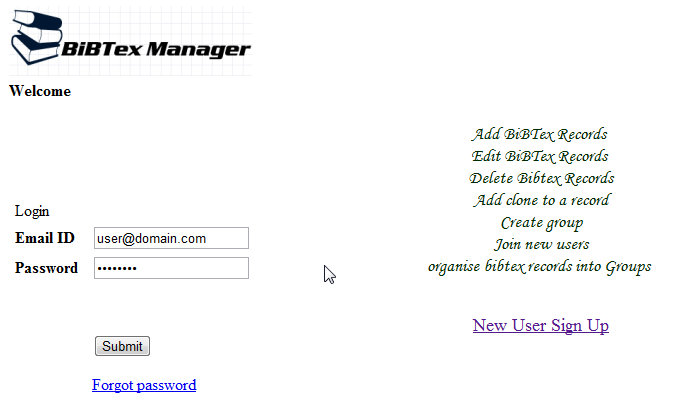
\includegraphics
			[scale=0.65]
			{images/LoginScreen.png}
		\caption{BibTeX Entry Manager Login Screen}
		\label{fig:RaviLoginScreen}
	\end{center}
\end{figure}

\begin{figure}
	\begin{center}
		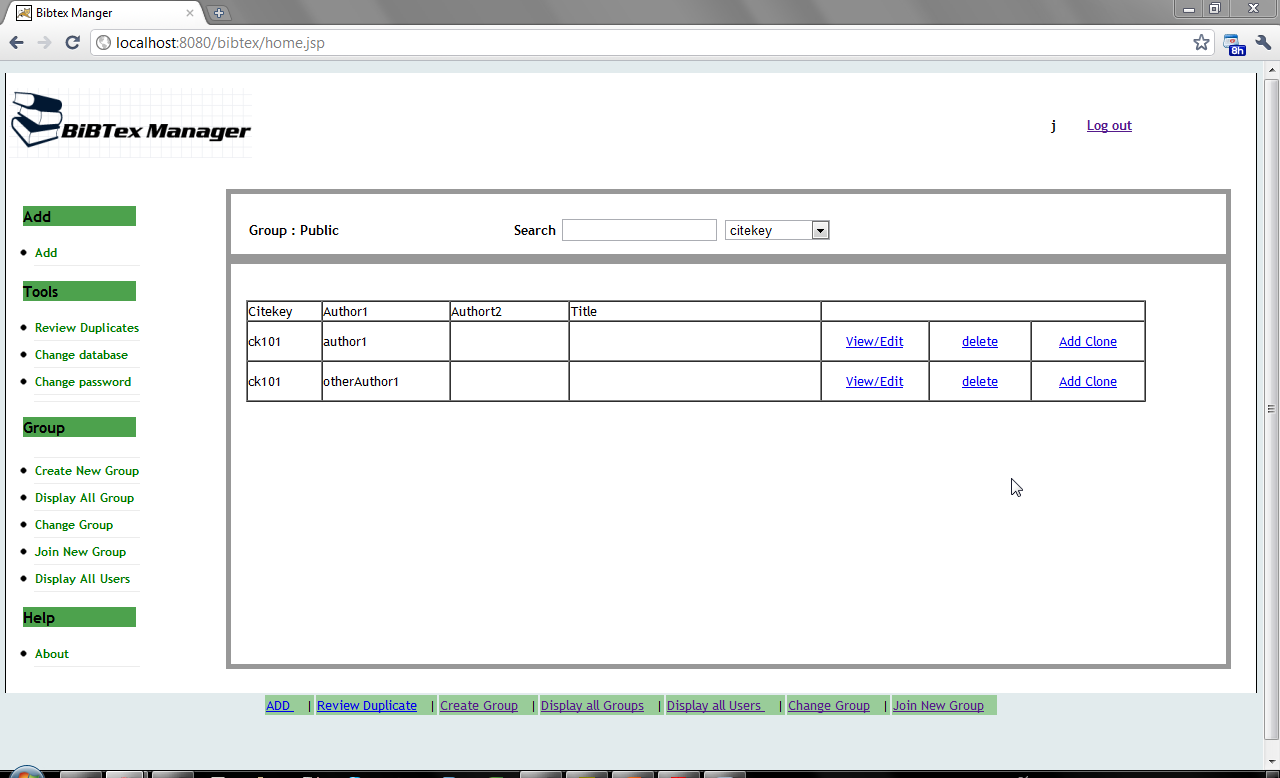
\includegraphics
			[scale=0.4]
			{images/RaviListScreen.png}
		\caption{BibTeX Entry Manager List Entries Screen}
		\label{fig:RaviListScreen}
	\end{center}
\end{figure}

The product has two navigation areas which contain different sets of commands in different orders, and changes across different pages. This can leave the user slightly overwhelmed and confused; consistency across pages would have defended against this issue and should be sought in the solution that is produced. 
In setting out to perform this background research, it was intended that the examiner would upload/open a file and perform further additions, modifications, deletions and searches across known entries from that initial file.  The lack of file import capability in the product was limited the consistency of the examination on this product, and was a significant shortcoming of the product. 

It is easy to deduce from the homepage what a user should click to add an entry to the system, though after an addition is performed, no message is shown to indicate success or failure of the operation.  It is clear that Nielsen's first heuristic \cite{NielsenHeuristics}\footnote{\label{nielsenH1} Nielsen's first heuristic says that the system should always keep users informed about what is going on. (Visibility of system status)} should be adhered to when designing future solutions to this problem.% don't think it is sufficient just to cite this web page, though they are listed here: http://www.useit.com/papers/heuristic/heuristic_list.html

After a break of perhaps twenty minutes in the examination, the user returned and reloaded the home page of the project, only to find that an error had occurred (a NullPointerException was thrown, resulting in a \gls{http} 500 error).  The error was not dealt with in a user-friendly fashion and reflects badly on the product.  The lesson to be learned here is that the product should deal with errors in a professional manner and not show exceptions on screen to users.

There is no `export' functionality so items cannot be taken out of the system and used directly in the \bibtex{} environment without first reconstructing the entry.  This is quite inconvenient for a user; the lesson to be learned from this is that basic functionality should be provided to ensure that the system is useful to a user.
The modification of an entry is relatively straightforward.  However, if a user wishes to change an entry's type after it has been saved to the database, they will be disappointed because the entry type is not a field that can be changed by any visible means without re-creating it in the database: users should be able to change an entry's type at any point after creation.

Another adverse feature of this product is its search capability.  It is difficult to deduce what state a search is in, given that there is no feedback to the user to say that a search is ongoing, complete, or otherwise.  This lack of feedback causes confusion and adds to the call for future projects and solutions to adhere to Nielsen's first heuristic. Unfortunately, there is no visible help menu or area to the product to help to describe how any of the functions behave. Such a menu would have been particularly helpful to assist with the search function, which is another concern that Nielsen addresses in his list of heuristics.  This lack of help or support is a shortcoming of the product and future projects should provide to avoid usability issues.

There is a provision for users to be able to switch to another database server from the one that they are using.  This might be helpful to some users, but there is potential for unnecessary replication across multiple servers.  It is also unclear from the user interface what database engines and schemas are supported by the system; this should be covered by a user manual or help system.

Entries can be categorised by users into different groups and allows a user to choose between groups currently in view \ref{fig:ChangeGroupScreen}.  This involves creating a group with a name and a description, changing to the new group and then adding entries to the group by the method previously used.  This is a helpful feature for categorising entries that do not yet exist, but a limitation of the system is that entries cannot be transferred from one group to another, and it means that they cannot belong to more than one group at any time.  Any future system implementing a grouping capability should allow entries to belong to many groups and should allow modification at any stage after addition to the set of entries, rather than restricting the flexibility of the system by failing to provide the functionality to make these changes.

\begin{figure}
	\begin{center}
		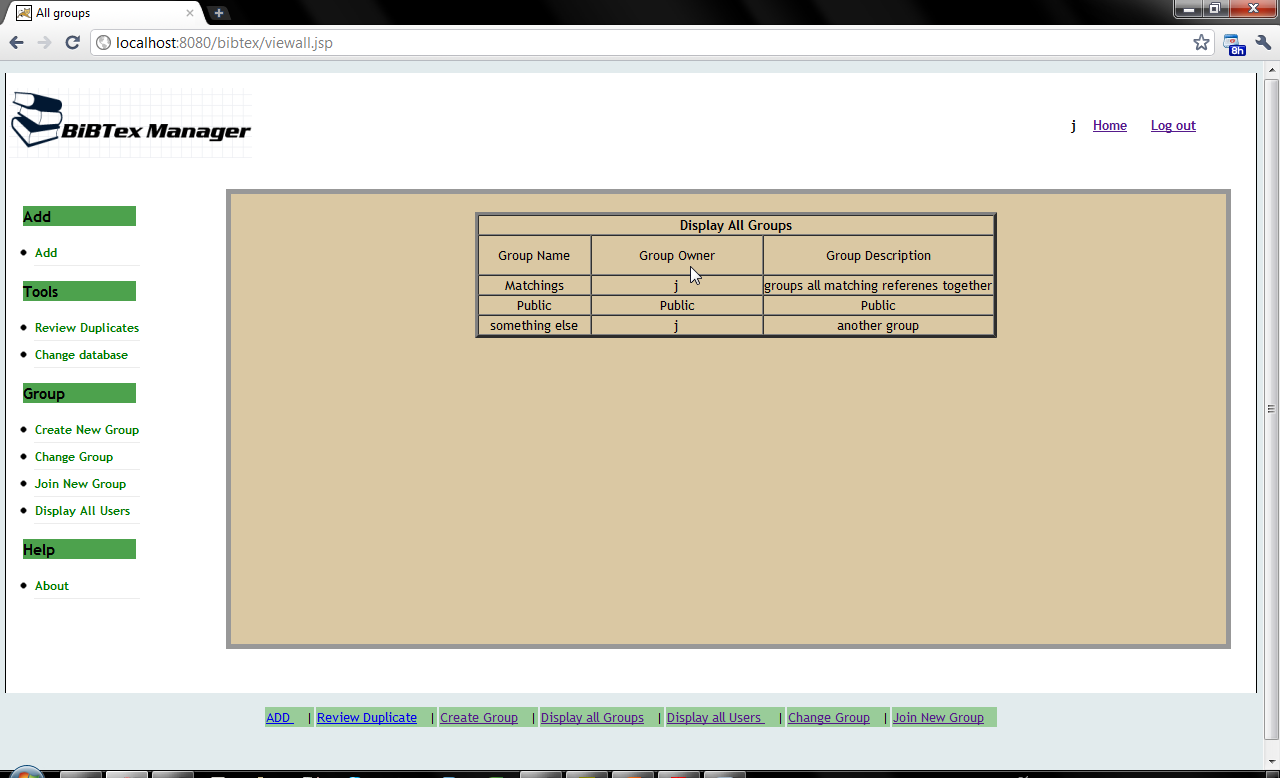
\includegraphics
			[scale=0.4]
			{images/ChangeGroupScreen.png}
		\caption{BibTeX Entry Manager Change Group Screen}
		\label{fig:ChangeGroupScreen}
	\end{center}
\end{figure}

The site allows users to access the same set of entries at the same time.  An issue that arises from this is that users may make changes to the same entry simultaneously, which could leave the entries in an inconsistent or incorrect state.  The solution deals with the problem by locking an entry until the first user to access it saves any changes they have made, or exits the viewing window.  This solution means that there can be absolutely no overlapping of interests when multiple people access the same entry.  An issue that arises from this method, however, is that if one user (user A) views an entry, then forgets to close the window, the entry is locked for a period of time.  When users B and C come to view it (perhaps with no intention of modifying it), they find that they cannot access it (see figure \ref{fig:RaviEditing}, leaving them unable to work and potentially frustrated while user A's time period of user A's viewing expires.  The system works on a pessimistic concurrency approach --- one that works on the assumption that clashes occur frequently --- and utilises a solution similar to the `locking' version control strategy.  This pessimistic strategy might not be optimal for the application and other approaches should be examined for future systems.

\begin{figure}
	\begin{center}
		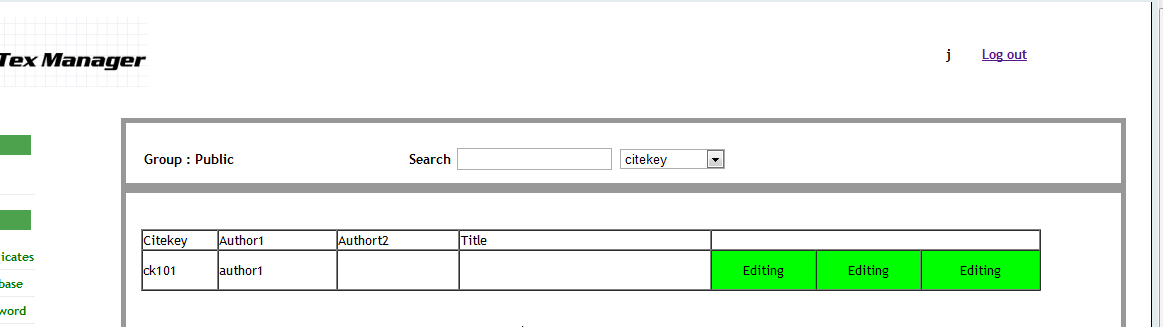
\includegraphics
			[scale=0.45]
			{images/RaviEditing.png}
		\caption{BibTeX Entry Manager -- Editing Notification}
		\label{fig:RaviEditing}
	\end{center}
\end{figure}

In summary, the examination of the \bibtex{} Entry Manager showed that:
\begin{enumerate}
	\item Consistency across pages is a highly important factor in the usability of the system; 
	\item Errors should be dealt with in a fashion that does not shed the product in a bad light;
	\item Import and export functionality should be provided to make the system useful;
	\item `Locking' an entry is too pessimistic for management of concurrent access to entries and another strategy should be found.
\end{enumerate} 


\subsection{BiblioScape}
BiblioScape is a desktop-based bibliographic data and note collection suite produced by CG Information.  It was created with the aim to ``build first class bibliographic software for the 21st century''.  It contains many tools which shall not be included in this examination as they are deemed to be surplus to requirements for the scope of the current project.\footnote{The system includes a forum and task list, among other things.} The live demo system is not as up to date as its current desktop counterpart (pictured on the website running on Windows 7), as the copyright notice at the foot of the home page dates back to 2002, where Windows 7 was released to the public in 2009 \cite{Win7Release}.

\subsubsection{Paradigm}
As part of the BiblioScape package, `BiblioWeb' was produced to ``address the needs of researchers in the age of the Internet'' \cite{BiblioWebWhy}.  It is a web-based version of their desktop program and allows users to access it through internet and Intranet connections and is the second product assessed in this series of three examinations.

\subsubsection{Ease of set-up}
A live version of the product was used on the BiblioScape website\footnote{The live version of the website is hosted at http://support.biblioscape.com:8001/}, so no comment can be made on the set-up process.

\subsubsection{Examination of product}
BiblioWeb has a clean \gls{ui}, and boasts a consistent navigation area at the top, whether a user is logged in or not.  Items in the menu at the top are spaced far enough apart that the interface feels uncluttered while also providing most of the basic options that a user expects of a reference management system, although edit, delete and export are not immediately apparent from the navigation bar, as can be seen in figure \ref{fig:BiblioScapeHomePage}. 

\begin{figure}
	\begin{center}
		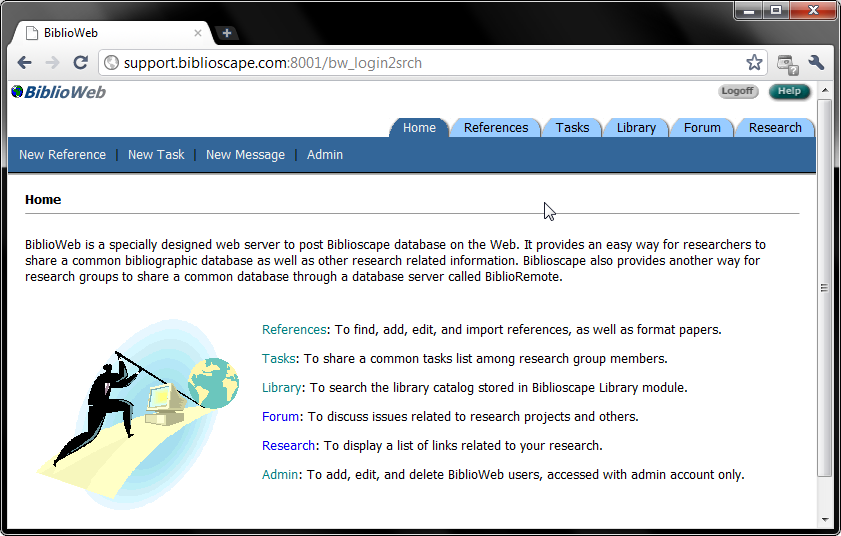
\includegraphics
			[scale=0.65]
			{images/BiblioScapeHomePage.png}
		\caption{BiblioScape Home Page (immediately after log-in)}
		\label{fig:BiblioScapeHomePage}
	\end{center}
\end{figure}

Another positive feature of BiblioWeb is that it has an intuitive interface and makes clear where one should go next when performing tasks.  On the other hand, one cannot obtain a list of all entries in the system, which means that a user might be forced to recall all information about an entry rather than rely on recognition; Nielsen \cite{NielsenHeuristics} specifies a heuristic guideline (his sixth out of ten) that a user's memory load should be minimised by making objects, actions and options visible.

BiblioWeb allows categorisation of references by use of folders (see figure \ref{fig:BiblioScapeFolderView}), much like the grouping function in the first project.  Some advantages that BiblioWeb's grouping method has over the first project's method include firstly that one can move many references at once from one categorisation to another, and secondly there is no need to delete an entry before reclassifying it.  It does appear, however, that references can only be in one folder at a time, which limits the flexibility of entries and perhaps allows redundancy in the database, where it could have been avoided by allowing an entry to belong to more than one category. 

\begin{figure}
	\begin{center}
		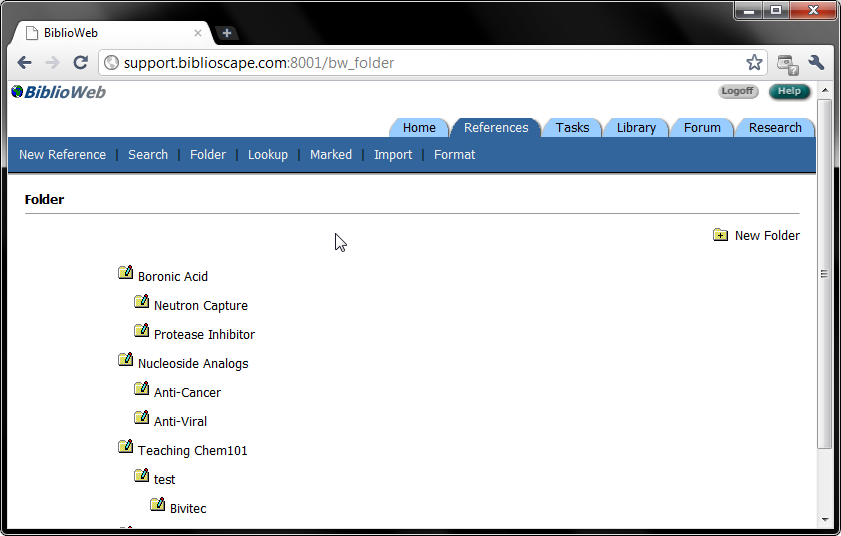
\includegraphics
			[scale=0.65]
			{images/BiblioScapeFolderView.png}
		\caption{BiblioScape Folder View}
		\label{fig:BiblioScapeFolderView}
	\end{center}
\end{figure}

Users' actions are clearly indicated when they are completed successfully, but the system falls down when incorrect input is supplied.  An example of this is explained presently: text was supplied to the `year' field to see how the system behaved with a string supplied instead of an integer.  Rather than displaying a helpful error message on the interface, the system navigated to a plain white page and displayed the word `EXCEPTION', followed by what was assumed to be a database exception.  As was the case in the first solution, the system did not handle errors and exceptions in a user-friendly way.  It is important to ensure that the system deals with problems in a professional and informative manner, so that a user can recover from their error --- something that Nielsen covers in his list of heuristics \cite{NielsenHeuristics}.

Perhaps the greatest asset of the BiblioWeb system has is its import function which boasts an enormous list of text and file formats, as can be seen in figure \ref{fig:BiblioScapeImportScreen}.  There are unfortunately not enough resources for this experiment to test all 201 of the formats, but it is safe to say that the system handles parsing of \bibtex{} entries well.  The system does not store the entries' types as would be expected of a \bibtex{} reference management package: rather than storing the reference type `Unpublished' as it was in the \bibtex{} file, it stored `Personal Communication', which is not accurate to the \bibtex{} format, and subsequently leaves the terminology open to misinterpretation by a user.

\begin{figure}
	\begin{center}
		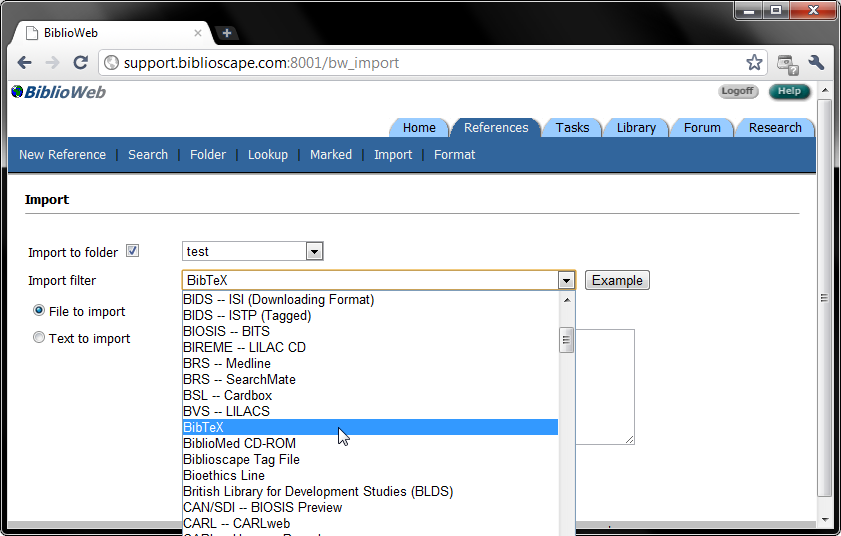
\includegraphics
			[scale=0.65]
			{images/BiblioScapeImportScreen.png}
		\caption{BiblioScape Import Page}
		\label{fig:BiblioScapeImportScreen}
	\end{center}
\end{figure}

The system's single greatest failure is that it does not support the export of entries to the \bibtex{} format.  This is a fatal flaw in terms of using the product with the main intended package of the project, \bibtex, although it does export to BiblioScape tag file, EndNote, RIS and Unix Refer formats, so can be used with their respective packages.

Therefore, overall, BiblioScape offered a clean, intuitive user interface and a vast array of import formats, but on the other hand failed to provide an export to the \bibtex{} format, was not consistent with the \bibtex{} entry types during storage, did not handle system errors well and was therefore not a suitable solution on its own.  Some of the lessons learned from this product can be taken forward into the production of a new system.

\subsection{\bibtex{} Manager}
\bibtex{} Manager, the last of the three products examined, is a reference manager specifically created for management of \bibtex{} entries.  It was written in Java by Mitesh Pravin Furia during 2009 as part of the requirements of the MSc IT degree at the University of Glasgow.

\subsubsection{Paradigm}
The product is a desktop-based application which can connect to a database, presumably to allow concurrent and multi-user access, though no user manual is included and it was not possible to test the feature.

\subsubsection{Ease of set-up}
The product was very easy to set up; it simply requires that a \gls{jre} is installed, which is obtainable from \url{http://www.java.com}.

\subsubsection{Examination of product}
The \gls{ui} to the system is well laid out and components of the interface are well spaced across the screen. The application follows the convention of many desktop-based applications and uses a menu bar at the top, containing the `File' menu, along with `Edit', `Tools' and `About'.  The menus remain consistent throughout use and are a solid go-to point for most pieces of functionality, which works in the application's favour.

The consistent menu is complemented by a consistent table area where currently loaded entries are displayed, as shown in figure \ref{fig:MiteshLoadedEntries}.  It is clear when there are no entries, as the area is greyed out slightly and the presence of entries in the system is also clear, thanks to the display of each entry as a row in the table.  An entry is selected by clicking on it, although it does not encourage a user to click by appearing to be clickable, as it has been styled to look like a display table.  McSweeney says that the ``features of an object should make it self-apparent how the object should be used'' \cite{affordance}, a principle which should be adhered to when implementing the resulting system of this study.

\begin{figure}
	\begin{center}
		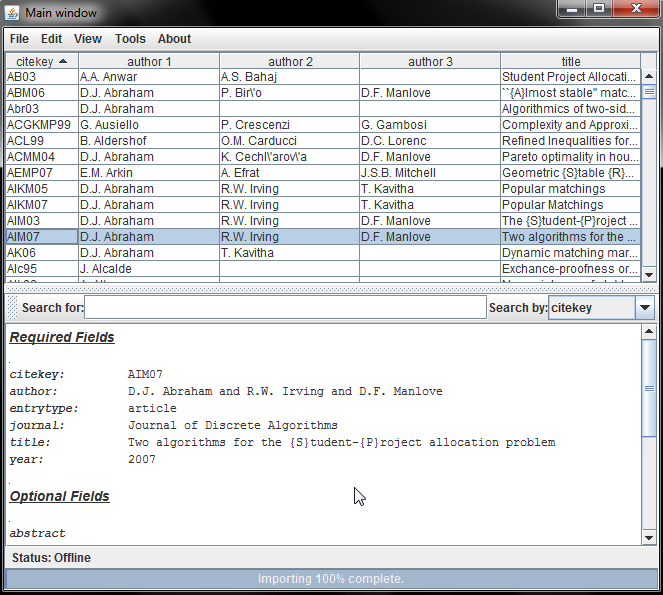
\includegraphics
			[scale=0.65]
			{images/MiteshLoadedEntries.png}
		\caption{\bibtex{} Manager with entries loaded}
		\label{fig:MiteshLoadedEntries}
	\end{center}
\end{figure}

There is no option to log in as a user, but there is an option in the `tools' menu to choose a database, as shown in figure \ref{fig:MiteshDatabaseScreen}.  This was assumed to be an implementation of multi-user access, but, as there was no user manual or help system, it was not possible to assess this aspect of the system.  It is important to document the features of the system if the actions to use it are not immediately clear, and help should be provided for complicated pieces of functionality.

\begin{figure}
	\begin{center}
		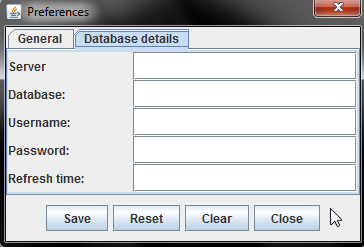
\includegraphics
			[scale=0.65]
			{images/MiteshDatabaseScreen.png}
		\caption{The database information input screen for the \bibtex{} Manager}
		\label{fig:MiteshDatabaseScreen}
	\end{center}
\end{figure}

The program deals with correct input successfully, and does not have any difficulty parsing correctly formatted files.  It gives some feedback for successful cases, though it would be helpful to know how many entries were successfully imported. When it is supplied with a file that it cannot deal with, it does not fail gracefully: a rather abrupt error is shown in a message box on the screen and gives no helpful message to the user, as shown in figure \ref{fig:MiteshFailedImport}.  If an error occurs, it is important to ensure that a user can recover from the error, which means that the program should give a meaningful message relevant to the context of the problem encountered.

A problem arises when there is incorrect user input or an erroneous entry is passed to the system.  When adding or modifying an entry, it is possible to submit and save an entry with some of the `required' fields left incomplete.  This would not be such a problem if the interface had some way of marking invalid or incomplete entries, but entries can be stored and subsequently exported to a file with no warning to the user that any invalid entry was encountered; a problem that has the potential to cause problems when the exported file is used with \bibtex{}.

\begin{figure}
	\begin{center}
		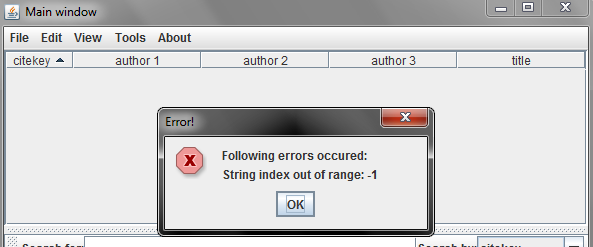
\includegraphics
			[scale=0.65]
			{images/MiteshFailedImport.png}
		\caption{The \bibtex{} Manager, having failed to import a file}
		\label{fig:MiteshFailedImport}
	\end{center}
\end{figure}

The product provides all of the `basic' functions that were outlined in the examination criteria (section \ref{examCriteria}) are available for use in the product, which is clearly a positive quality of the software.  Two further functions that are provided by the system include `Add Clone', which intentionally duplicates an entry	to reduce the need for retyping a similar entry's details and `Review Duplicates', a provision to compare entries with the same cite key side-by-side with the aim of removing duplicate entries.

In the \bibtex{} format, cite keys are delimited from the rest of an entry by a comma; the cite key field in this solution allows commas to be entered which, left in the field, can lead to errors when the resulting file is used.  The `year' field, on the other hand, is validated and allows only numbers to be stored in the field (see figure \ref{fig:numbersOnly}), which is a good example of the system enforcing correct entry with feedback through a clear error message. 

\begin{figure}
	\begin{center}
		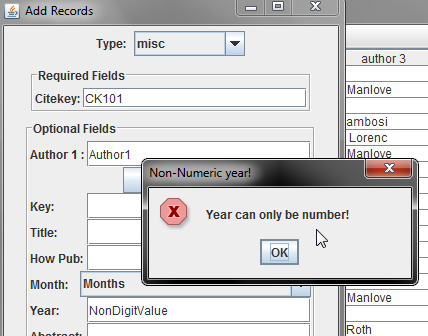
\includegraphics
			[scale=0.65]
			{images/MiteshnumbersOnly.png}
		\caption{Rejection of non-numerical values by the \bibtex{} Manager}
		\label{fig:numbersOnly}
	\end{center}
\end{figure}

In summary, The \bibtex{} Manager is a good solution to the problems faced by authors, boasting a well-spaced, menu-driven, consistent user interface which provides all expected functionality.  Its shortcomings include that some fields are not validated correctly, the entries in the table do not look clickable, feedback for file parsing errors are not helpful and invalid entries can be stored and exported without warning.

\section{Summary}
This chapter examined three products according to three sets of examination criteria. Several lessons, to be kept in mind for the duration of the project, were learned during the examinations, and are summarised presently:
\begin{enumerate}
	\item Make it as easy for a user to set up the program as is possible;
	\item Provide feedback to users when actions have been performed;
	\item Keep errors under control where possible and deal with them neatly when the user needs to be notified;
	\item Allow an existing entry to be moved between categories at any time;
	\item Control access to entries in a way that does not impede the progress of other users;
	\item Keep pages consistent to reduce cognitive load on a user;
	\item Support \bibtex{} file import and export;
	\item Make the product easy to navigate to;
	\item Provide `basic' functionality to ensure that the system is useful to a user;
	\item Allow a user to be able to change an entry's type at any point;
\end{enumerate} 

The next chapter discusses the requirements engineering phase of the project, while keeping in mind the lessons learned in this chapter.
\glsresetall{}
\chapter{Requirements Engineering}
\label{reqs}
Therequirements engineering chapter gives a vision of what the project aims to provide and to whom: it identifies stakeholders in the project and analyses their areas of interest, before providing a list of functional and non-functional requirements, including a prioritisation of stakeholders and requirements.

\section{Stakeholders}
A stakeholder is a person or group of people who have an interest in the resulting software from this project.  Several (groups of) stakeholders of the project were identified: 

\revisit --- are there any other interests that have been missed?

\begin{enumerate}
	\item Users of \bibtex{} are the intended audience of the software product created by this project, particularly academics and other technical authors --- they are therefore stakeholders in the project.  Their main interests in the product lie in how usable the product is and the accuracy and validity of its outputs;
	\item As an author, the project supervisor's interests are a superset of the first group's interests, and also include ensuring that the student under supervision develops as an individual;
	\item The student developing the project is interested in furthering technical and professional expertise, as well as providing a product which surpasses expectations of the project supervisor and other stakeholders;
	\item Students who undertake this project in the future may be interested in the positive qualities of and the lessons learned by this project.
\end{enumerate}

\subsection*{Prioritisation}
The stakeholders are listed in order of priority, with justification for their positioning:
\begin{enumerate}
	\item Stakeholders 2 and 3 hold the highest priority as they are directly involved with the development of the project and have the most to gain if the project is successful. \revisit Wording.
	\item Stakeholder group 1 hold the second highest priority; potential users must be consulted when evaluating the product
	\item Stakeholder group 4 may have some interest in the way that the project was constructed, what it achieved, as well as lessons that were learned and mistakes to be avoided.  Their concerns are of a lesser importance, though they should still be considered.
\end{enumerate}

\section{Functional Requirements}
\label{funcReq}
A functional requirement is a task that the software must allow a user to perform.  The tool should provide management of \bibtex{} records, and should specifically allow users to:
\begin{enumerate}
\item Add an entry;
\item Edit an entry;
\item View entries;
\item Delete an entry;
\item Undo the deletion of an entry;
\item Perform a simple search on entries;
\item Perform an advanced search on multiple fields of entries;
\item Import entries from a file uploaded by a user;
\item Export entries to a file for download by a user;
\item Users should be able to group entries to assist with the organisation of citations;
\item Items should expire (deleted items should be removed entirely) after a period of time;
\item Users should be able to review and manage duplicate\footnote{A pair of duplicate entries have matching cite keys.} entries.
\end{enumerate}

\section{Non-Functional Requirements}
\label{nfReq}
A non-functional requirement is a rule that the software must adhere to, but is not a specific action that a user can perform.  The tool should adhere to the following non-functional requirements:
\begin{enumerate}
\item Interaction with the system should take place through a web-based interface;
\item The server-side application is not required to be portable;
\item The client-side (web interface) should be accessible from major (*nix, Windows, Mac) operating systems under the three most widely-used browsers (Mozilla Firefox, Google Chrome, Microsoft Internet Explorer) \cite{w3cBrowserStats};
\item Entries should be stored in a central database;
\item The system should allow multiple users to collaborate on a collection of \bibtex{} entries;
\item The system should be usable by the target audience, users of the \LaTeX{} typsetting tool;
\item The system should authenticate users;
\item The system should allow various levels of access to users with different
privileges;
\item The system should be able to handle concurrent access by multiple users in such a way that it facilitates their collaboration on the centrally stored set of references;
\item Only valid entries\footnote{To say that an entry is `valid' means that it has all of its required fields populated} should be stored by the system;
\end{enumerate}

\section{Prioritisation}
The functional requirements laid out in section \ref{funcReq} are prioritised (highest first) as follows:
\begin{enumerate}
	\item Items 1, 2, 3, 4, 6, 8 and 9 have the highest priority and are defined as the `Basic' functionality that must be implemented in the project;
	\item Items 5, 7, 10, 11 and 12 hold a lower priority than the items in (1) and will be implemented if time permits.
\end{enumerate}

It is important to point out at this point that the system must adhere to the non-functional requirements laid out in section \ref{nfReq}, all of which are high priority with the exception of item 7.

\section{Summary}
The software artefact must adhere to the requirements set out in this chapter.  Prioritised requirements have been set out and should be tackled in order of necessity. \revisit --- extend summary.
\glsresetall{}
\chapter{Design}
\label{design}

This chapter sets out to describe the approach taken to designing a software solution for the requirements discussed in the previous chapter.  It outlines the key concepts behind the user interface design, after which it discusses the different approaches taken in structuring the classes used to model the problem, before going on to describe the database tables that are used.

The chapter begins with a description and depiction of the architecture used, before going on to discuss the rest of the design with the requirements and lessons learned from background research in mind. 

\section{System Architecture}
Non-functional requirement 1 states that interaction with the system should take place through a web-based interface.  This requirement fits well with the client-server model: a set of clients that call on the services offered by a server (or set of servers), facilitated by a network \cite{sommerville}.  The approach taken by the solution is illustrated by the \gls{aod} in Figure \ref{fig:aod}, which is intended to bring the system to life for a reader.

This architecture could, with some reconfiguration, be scaled up to run on multiple servers, including the possibility of separating the database onto another machine, as well as replicating the application across different load-balanced systems.  It was sufficient for deployment of the project to centralise all of the functionality to one piece of hardware, and a \gls{vm} was produced so that it could be emulated on other hardware.

\begin{figure}
	\begin{center}
		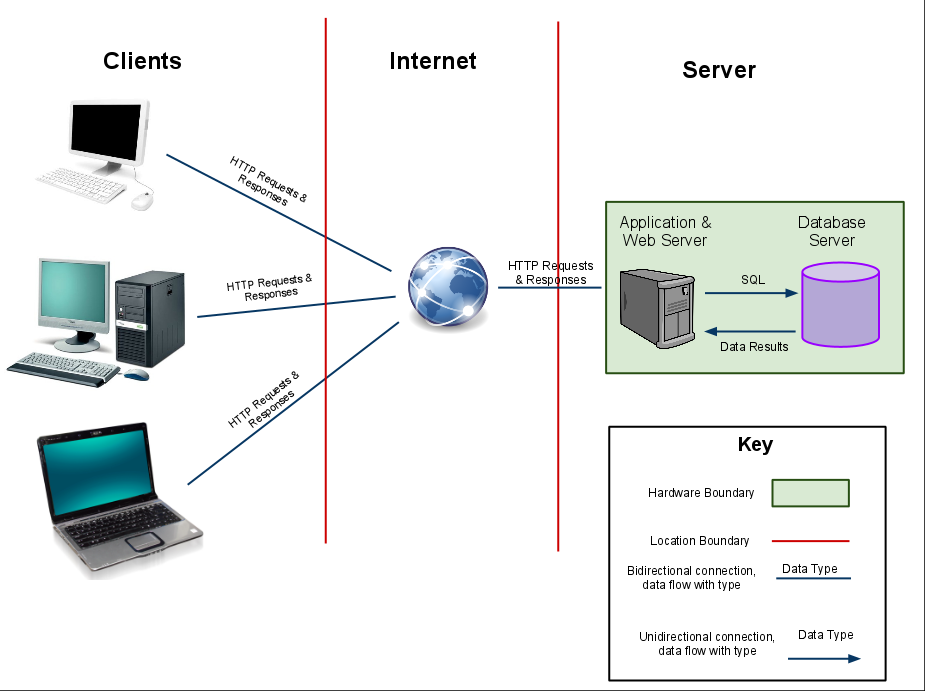
\includegraphics
			[scale=0.45]
			{images/ArchitectureOverviewDiagram.png}
		\caption{High Level Architecture Overview Diagram}
		\label{fig:aod}
	\end{center}
\end{figure}

\begin{figure}
	\begin{center}
		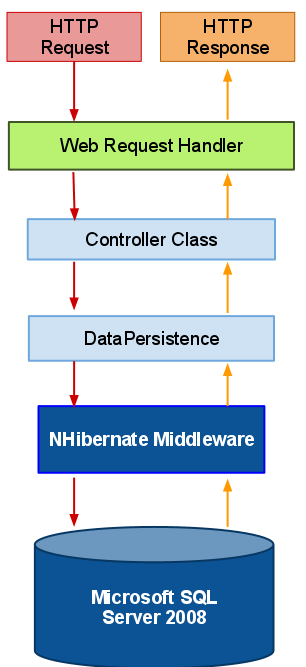
\includegraphics
			[scale=0.45]
			{images/DataFlow.png}
		\caption{Diagram showing high-level data flow between components}
		\label{fig:dataFlow}
	\end{center}
\end{figure}

\section{Web Interface Design}
\label{uiDesign}
The interface design was conceptualised around the idea of a clean, consistent and intuitive interface, in line with the requirements and background findings.  It was important to take account of Fitts' Law, the observation that the smaller a target is, the harder it is for a human to point at and act upon accurately \cite{fitts} (particularly in the 2-dimensional space of a screen \cite{fitts2d}), and to adopt a common sense approach when deciding how large or small clickable items should be.

\section{Class Designs}
This section discusses the class designs as they evolved over different versions of the program, as well as reasons for changes.  Each version is named after NASA Space Shuttle orbiters in chronological order of when they entered service.

An \gls{oo} approach was taken with the project, as the entries that were to be saved mapped well to the concept of an object, and because the \cs{} language is a natively \gls{oo} language.  The \cs{} language is discussed in more detail in Section \ref{csharpDiscussion}.


\begin{figure}
	\begin{center}
		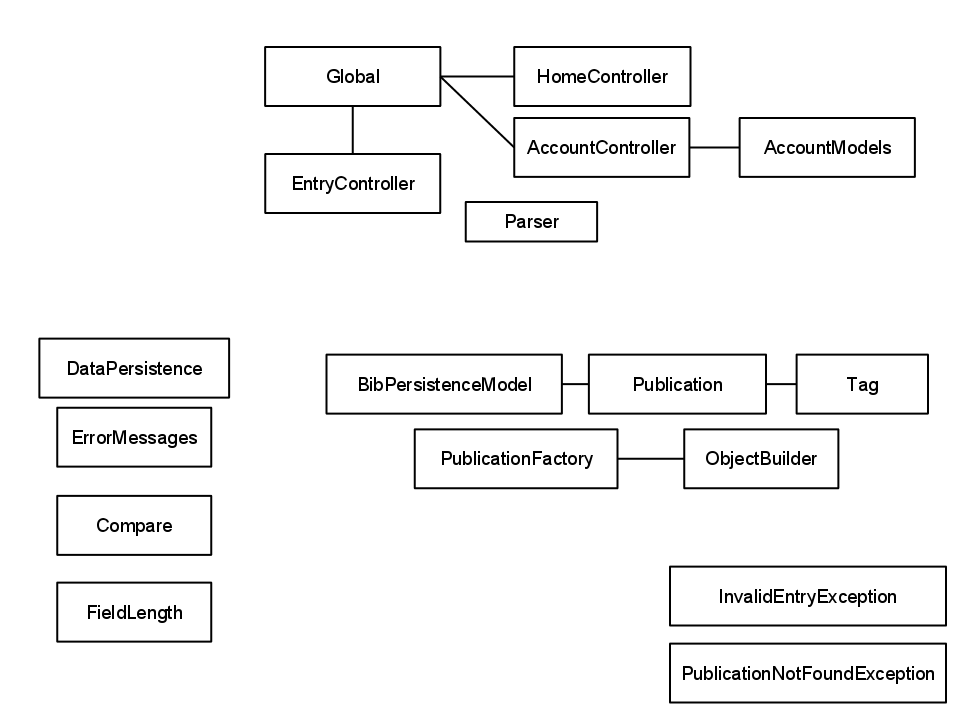
\includegraphics
			[scale=0.45]
			{images/OverallClassDiagram.png}
		\caption{UML Class Diagram showing all classes}
		\label{fig:OverallClassDiagram}
	\end{center}
\end{figure}


% reset mvc acronym.
\glsreset{mvc}
\subsection{Model View Controller}
The application's design is heavily based on the \gls{mvc} architecture.  The data model and database interaction are all taken care of in core classes, namely the \texttt{DataPersistence} and \texttt{Publication} classes.

\subsection{First model version (V0.34 - Columbia)}
\label{columbia}
The approach of the first model version was heavily based on the approach of Mitesh Furia; it was seen as advantageous to reuse the code from his project as much as possible, to reduce development effort and increase the output functionality at the end of this project.  With this aim in mind, the class design for the initial model was heavily structured around his approach.  This approach did not survive the entirety of the project; as development progressed, it became apparent that the design would need to be refactored and streamlined, as discussed in Section \ref{designChallenger}.  The main surviving item from Mitesh's solution was the file parser, which was modified to suit the \cs{} language (from Java) and to provide further feedback to users.

The initial class design consisted of one class per entry type (see Figure \ref{fig:ColumbiaClassDesign} --- an example list of which fields are required and which are optional are shown in Figure \ref{fig:ArticleFields}).  The main focus behind this approach, aside from following Mitesh's successful approach, was to take advantage of a feature of the \gls{net} Framework called Attributes, which can be used effectively for validation.  Attributes provide the ability to associate extra information with each member variable of a class; as an example, the `required' attribute can be used to enforce the requirement to include data in a field for it to be valid.  This approach worked well for this version of the model, boasting excellent robustness to poor or erroneous user input as well as excellent feedback to users through the provision of error messages assigned by the required attribute.  Optional fields were included as member variables, and took advantage of the `DisplayName' attribute. The \gls{net} framework allows automatic generation of labels for web pages, so when a member name doesn't have spaces it results in poor display on the interface.  An example of a member variable name lacking spaces is the field `howpublished': it is more readable and therefore more user friendly when the field is displayed as `how published', which is achieved as shown in Figure \ref{fig:displayName}.

\begin{figure}
	\begin{center}
			\lstset{language=CSharp} 
			\begin{lstlisting}
  // The attribute
  [DisplayName("Book Title")]
  // The member name with no spaces
  public virtual string Booktitle { get; set; }
			\end{lstlisting}
		
\includegraphics{images/displayNameOnInterface.png}
		\caption{Use of a field name attribute to display a field name differently}
		\label{fig:displayName}
	\end{center}
\end{figure}

\begin{figure}
	\begin{center}
		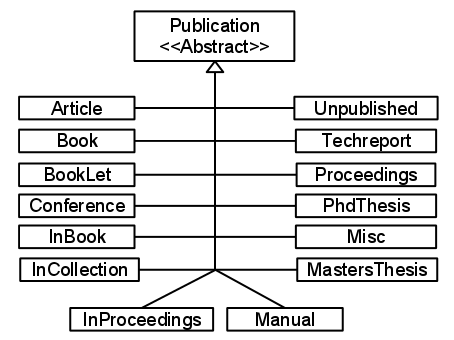
\includegraphics
			[scale=0.6]
			{images/ColumbiaClassDiagram.png}
		\caption{UML Class Diagram of the Columbia Model}
		\label{fig:ColumbiaClassDesign}
	\end{center}
\end{figure}

\begin{figure}
	\begin{center}
		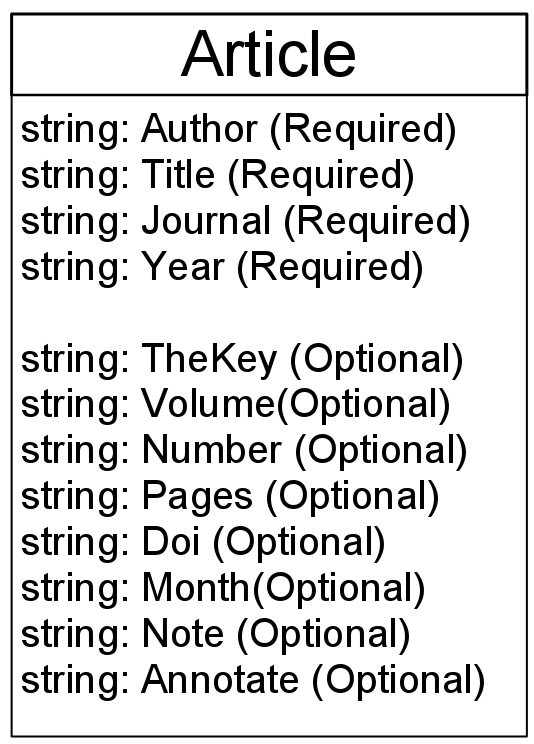
\includegraphics
			[scale=0.3]
			{images/ArticleFields.png}
		\caption{UML Class Diagram showing the required and optional fields for the `Article' entry type}
		\label{fig:ArticleFields}
	\end{center}
\end{figure}

Each entry type was a subclass of the abstract superclass \texttt{Publication}, which contained fields common to all entry types, namely: Id, an int identifier; CiteKey, a string intended to be unique to an entry, but not usable as an identifier in the database, allowing duplicate entries to exist in the system; Owner, the username of the user who created the entry in the first instance; along with Abstract, a string field which was to be optional to all entries.

As the class was designated `abstract', the enforcement of rules associated with the concept\footnote{Designating a class `abstract' means that an instance of it cannot be directly created, but an inheriting concrete (antonym of abstract) can be instantiated.} were used to the advantage of the developer: several methods, which were to be relied on and required by the controller classes, were added as abstract methods to the Publication class.  These abstract methods included two methods which converted an entry to a string representing the entry as a row in a \gls{html} table, both with and without hyperlinks to the amendment page for the entry.


\subsection{Second model: V1.0 - Challenger}
\label{designChallenger}
The Challenger model was the model adopted in the final (deployed) version of the product.  This is the model that is discussed during the implementation chapter (Chapter~\ref{impl}).

Columbia's design presented a few problems for development and performance on the system, as was discovered after implementation:
\begin{enumerate}
	\item 14 entry types meant 14 tables and 14 queries to search for an entry or retrieve all entries, which had a serious impact on performance;
	\item Identifiers were unique to each table only, and did not necessarily identify an entry from all others, which resulted in problems with access by the application.
\end{enumerate}

To solve these problems, a large refactoring took place to reposition all entries' fields in the top-level class \texttt{Publication}.  This reduced the class diagram for the model from as shown in Figure \ref{fig:ColumbiaClassDesign} to as shown in Figure \ref{fig:ChallengerClassDiagram}

\begin{figure}
	\begin{center}
		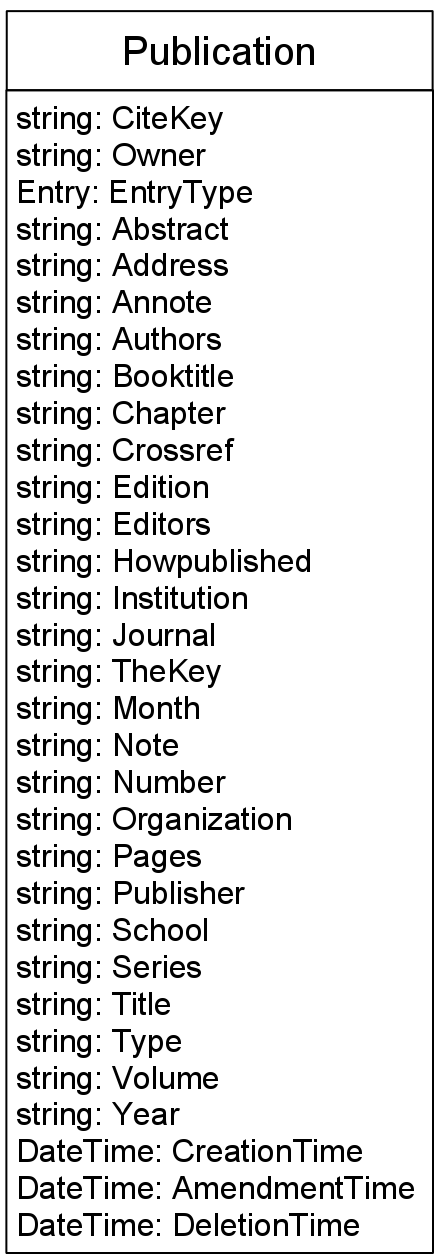
\includegraphics
			[scale=0.3]
			{images/ChallengerClassDiagram.png}
		\caption{UML Class Diagram of the Challenger Model}
		\label{fig:ChallengerClassDiagram}
	\end{center}
\end{figure}

This directly maps to the database model

Single table for all entry types:\\
why\\
what improved?\\
 - faster search\\
 - IDs all in one place - less complicated - don't need to kow what an entry's type is before searching it\\

\subsection{Third (proposed) model: V2.0 - Discovery}
\label{designDiscovery}
Discovery was intended to add a feature called `tagging' to the system.  \\
Specifically, this was to involve a many-to-many mapping from \texttt{Publication} to \texttt{Tag}


\section{DB Design Diagram}
content

\glsresetall{}
\chapter{Implementation}
\label{impl}
The implementation chapter covers the technologies, techniques and patterns applied to this project.  Many of the contents were encountered were encountered during a summer placement at a technology company in Glasgow between levels 3 and 4.  

\section{Technologies Used and Discipline}
This section examines the technologies used in the implementation of the project and the discipline that was adhered to during development.

\subsection{Microsoft .NET Framework}
The Microsoft .\gls{net} framework is a platform for development, deployment and running of web services and applications \cite{whatIsDotNet}.  It provides a \gls{clr}, similar to the \gls{jvm} in Java  This project took advantage of \gls{asp}.\gls{net} \gls{mvc} 2.  

Microsoft's .\gls{net} framework was used as a result of encountering the technology during the summer placement.  The developer saw the opportunity of learning more about and working with the framework when the project was successfully assigned to him.  Given that one of the aims of the summer placement was to learn .\gls{net} development, and that this aim was not completely achieved \cite{summerPlacementReport}, the developer chose to maximise exposure to the technology by working with it for the duration of the project, and adding an aim to learn the framework to the project goals.  It may appear that this was a short-sighted decision, but there are many other benefits to using this technology, including:
\begin{itemize}
	\item There is an active developer community on the web\footnote{The community's forums can be found at \url{http://www.asp.net/community} and a large proportion of active users of the Stack Overflow community focus on C\# and .\gls{net} topics --- 3 of the top 8 tags are directly related to the project's domain --- \url{http://stackoverflow.com/tags} (by observation)}, so issues pertaining to development using the framework can be solved by turning to this well-grounded knowledge base;
	\item The \gls{mvc} aspect of the project, if strictly adhered to by the developer, provides great separation of concerns between the place that information is stored, manipulated and viewed;
	\item The framework allows for portability to other client machines with very little in the way of model adjustment. For example, if a requirement for a mobile or tablet application developed, it would simply be a case of adding the functionality for that device, rather than having to reimplement the model for a particular piece of hardware.
	\item Applications can be deployed, with some adjustments, on Linux machines using the Mono (open source) software platform \revisit - awaiting help from Gregg
\end{itemize}

\glsreset{oo}
\subsection{C\#}
C\# is an \gls{oo}, garbage-collected programming language which has roots in the C family of languages.  It is standardised language (ECMA-334 and ISO/IEC 23270) with compilers available for unix based systems (using the `Mono' compiler) and Windows systems (using Microsoft's C\# compiler for the .\gls{net} Framework) operating systems, which both conform to the ECMA and ISO/IEC standards \cite{monoStandardised} \cite{csPL}.

C\# was used over the other .\gls{net} languages (of which there are at least 30) \cite{csUnleashed} because the developer wanted to become familiar with the language having encountered it and used it while on summer placement.

\subsection{NHibernate and Fluent NHibernate}
\label{nhibernate}
NHibernate is a port of the Hibernate object/relational mapper to the .\gls{net} framework. In essence, it provides mapping from objects to relational tables, which allows a developer to concentrate on functionality and usability rather than spending time writing \gls{sql} scripts. Queries are generated by NHibernate middleware and passed to the database which, after execution, accumulates any results into objects directly manipulable by C\# code. 

An example of how this technology helps and works is described presently: Let's assume that a series of valid entries have been created in the database and that a user has issued a request to view the details for one of them, with the \gls{id} 3.  Sample code to fetch the publication associated with this Id and return it as a usable object is shown in figure \ref{fig:fetchPubCode}.

\begin{figure}
	\begin{center}
			\lstset{language=CSharp} 
			\begin{lstlisting}
	public static Publication GetPublication(int givenID)
	{
	    // Get an NHibernate session with the database
	    ISession ses = GetSession(); 
	
	   	// LINQ query used to construct SQL query in middleware
	    IQueryable res = from pubs in ses.Linq<Publication>()
	                     where pubs.Id == givenId
	                     select pubs;
	                        
	    // pull the first item from 'res' 
	    Publication thePublication = res.First();
	    
	    return thePublication;
	}
			\end{lstlisting}
		\caption{Code to fetch a Publication by ID}
		\label{fig:fetchPubCode}
	\end{center}
\end{figure}

The code in figure \ref{fig:fetchPubCode} returns the publication for manipulation in code; persisting changes made to the entry after manipulation (or saving an entry for the first time) is very simple, as shown in figure \ref{fig:storePublication}.

\begin{figure}
	\begin{center}
			\lstset{language=CSharp} 
			\begin{lstlisting}
	// saves the item for the first time if it does not yet exist
	// or updates the entry if it already exists (pubVar is of type 'Publication')
	pubVar.SaveOrUpdateInDatabase();
			\end{lstlisting}
		\caption{Code to store a publication after creation or modification}
		\label{fig:storePublication}
	\end{center}
\end{figure}

The NHibernate software itself is highly valuable in terms of time-saving potential and has been used across thousands of successful projects \cite{NhUse}.  The only issue with using it in its raw form is that mappings from the project's classes to relational entities have to be written in \gls{xml}, a language prone to errors often left unnoticed until runtime.  A better solution is to use the Fluent NHibernate extension, which provides developers with the ability to map the classes in code.  The major benefit of this scheme, aside from compile-time error checking, is that all code using is strongly-typed; combine this with the powerful \gls{msvs} \gls{ide}, and implementation for the data model can be quite rapid --- particularly when in the hands of an experienced developer.

Another reason for using this technology was that it was used within the summer placement, but it was not encountered or worked with to any great extent.  \revisit Curiosity fuelled, the developer wanted to expand his knowledge in the technology in both breadth and depth by adopting these technologies within the project.

There was a risk, when employing this technology, that unfamiliarity would lead to hindrance rather than benefit by employing it.  Before automatic generation of database scripts for interactions can take place, Fluent NHibernate has to be instructed what to map and how to map it.  This was not something that the developer had encountered before; the risk was that learning how to map the classes to entities correctly would take too much time and have an impact on the progress of the project.  To mitigate the impact of the risk, a deadline was agreed between the developer and the supervisor: if, by the final day of term in semester 1, the mappings were not working correctly, then NHibernate as a data solution would be abandoned and standard \gls{sql} queries would be used.  As it turned out, the mappings were finalised on the afternoon of the deadline, so NHibernate use went ahead.  The aforementioned benefits of NHibernate were noticed during development, and some experience was gained in the implementation and use of object/relational mapping in practice.

\subsection{Subversion}
\label{svn}
\gls{svn} is a centrally-stored version control system which records every change ever made to the files and directories in the file repository \cite{CFP04c1}.  It is useful to be able to centralise the code repository and to be able to synchronise different workstations with the most up to date version of code and documents, as well as allowing the logging and comparison of different versions of the code.  Each time information is updated in the repository, it is said to have a new revision -- a process also known as `committing' changes.  It was decided early in the project that a repository would be used to mitigate the risk of fire, flood, theft, and hard drive corruption by hosting the repository in a different physical location to the main work environment, the developer's laptop.  

\gls{svn} was used to control different versions of the code and to take snapshots of the project in the form of \gls{svntag}s \cite{CFP04c4}, as well as normal revisions.  It was originally hosted on the School of Computing Science network because it was accessible from outside the School's network of computers\footnote{access was facilitated by the School's \gls{ssh} gateway, \texttt{sibu.dcs.gla.ac.uk}}, because there was sufficient storage space provided by the School and it had no financial cost.  As part of the effort to ensure good software engineering practice, \gls{ci}\footnote{See Section \ref{continuousIntegration} for an explanation of what it is and why it was used} was to be used with the project, again after encountering it while on summer placement.  Unfortunately, there were problems in configuring the  \gls{ci}  software to access the \gls{svn} repository through the gateway; as a result of this, on the 16\^{th} of November 2010, the repository was moved to another free host, SourceForge, an open-source software project hosting provider.  Along with \gls{svn} repository hosting, SourceForge provides tools for management of software projects, including a bug tracking tool (see Section \ref{bugTracking}).  Crucially, the SourceForge repository was accessible by the \gls{ci} software, allowing the \gls{ci} process to take place.

The \gls{svn} client in most cases was TortoiseSVN, as development was to take place on a windows environment.  AnkhSVN, a secondary client, was also used as it integrated with the \gls{msvs} \gls{ide}. 

The change log from the \gls{svn} repository is included as an appendix\revisit; the repository can also be browsed on the SourceForge website at \url{http://bibman.svn.sourceforge.net/}

\subsection{Bug Tracking}
\label{bugTracking}
Bug tracking is, as the name suggests, the tracing of the status of bugs that have been discovered in a system, used primarily to ensure that bugs which are found are dealt with or logged in a release.  It is another concept that was encountered while on summer industrial placement, and it struck the developer as an advantageous \gls{case} tool to utilise in this project.

The bug tracker was used when a bug was encountered that was not going to be fixed at the time of the discovery; the developer wanted to apply use of the bug tracker intelligently so that it was always going to be a help, and not a bureaucratic hindrance to development.  Bugs that were found were created in the system and given a priority, marked initially as `open' to symbolise that they had not yet been dealt with.  When a bug had been dealt with and the developer had verified that it was no longer an issue, it was marked as `closed', and remained in the system for traceability, should a similar issue crop up.  As a rule of thumb, a comment was recorded to say firstly what the problem was, secondly what the fix was and thirdly which \gls{svn} (see section \ref{svn}) check-in fixed the issue so that one did not need to trawl through logs in \gls{svn} to find the fix, should they need to revisit it.\\ \revisit - want to check wording of this paragraph when I'm not tired.

The software used was BugTracker.NET -- a free, open-source, web-based bug tracker.  Having encountered this particular product and worked with it for three months, the developer thought it wise to stick to familiar ground and employ the same product.  The developer used hardware running at home to deploy BugTracker.NET and used it until a server failure in late January 2011.  As the hardware was no longer reliable to host the software, the decision was taken to switch bug tracking software to SourceForge's Bug tracker, which worked in a similar way.  Bugs from the old system (both open and closed) were transferred to the new site and remain there now for traceability and reference. \\

\section{Development Environment}
\label{devEnv}
Most of the development took place on the developer's laptop, a MacBook Pro dual-booted with Windows 7 Professional.  Some development took place on a second developer machine when the laptop was unavailable.

The main development environment was Microsoft's Visual Studio Professional 2010 (\gls{msvs}), provided by the School's \gls{msdnaa} agreement.  This was the same environment used while on summer placement, so the developer was familiar with the tools in the \gls{ide}.

The database product used was \gls{msss} 2008 Developer Edition, again provided by the School's \gls{msdnaa} agreement. The management suite included with the product was again used while on summer placement, and the developer was familiar with the tools in the program.

ReSharper is a productivity plug-in for \gls{msvs}.  It provides code inspections, code analysis, one-click unit test runs, project-level refactorings and many more assistive features. A licence for the product was bought during the summer placement and was used extensively throughout the development of the software article.

Python IDLE and Notepad++ were used to manipulate code quickly and effectively: Python IDLE for its scripting functionality and Notepad++ for its macro capabilities and excellent search and replace by regular expression function.

TortoiseSVN and AnkhSVN were both used as discussed in section \ref{svn}.

\section{Reuse of Code}
\label{codeReuse}
Code reused within project \\
Code reused from other projects \\
 - pre tested
 - see somerville for more info.

Benefits of code reuse:
\begin{itemize}
	\item the reduction of maintenance overheads of having to test the same code in multiple places
	\item 
\end{itemize} 

Disadv/risks:
	bugs may exist if not widely used or well tested
	code may be less readable if not familiar with it
	

\section{Patterns}



\section{Data Model}
The design of the Data Model is discussed heavily in chapter \ref{design} 
Discuss implementation of data model, implementation of database persistence. centralised persistence information - single section of code + benefits.
The data model, as mentioned in section \ref{nhibernate}, is implemented using NHibernate.  
Discuss fields in publication table. Mention creation/modification/deletion times and what they are used for
ID field vs cite key
owner


\subsection{Refactoring}
changes to model from 0.34 to 1.0


\section{Controller}
Home controller
Account Controller
Entry controller:
 - Same page for add and amend
 - discuss import
 - 
Discuss handling of requests


\section{Web Service}
The project has several areas which are performed by \gls{ajax} interactions with the system.

Following facebook's highly successful use of \gls{ajax} in their user experience
Delete by AJAX\\
search\\
'what is new'\\
'what is amended'\\
'what is deleted'\\




\section{View}
\glsreset{ui}
\subsection{Consistency}
The consistency sought in the design of the product (see section \ref{uiDesign}) of the site is a result of careful consideration of what should be consistent across all pages, as highlighted in figure \ref{fig:pageLayout}:

\begin{figure}
	\begin{center}
		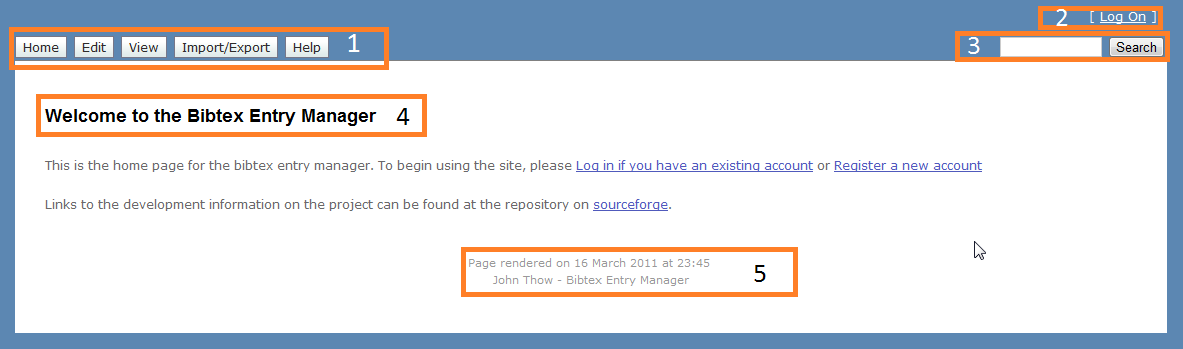
\includegraphics
			[scale=0.5]
			{images/PageLayout.png}
		\caption{Annotation of a page}
		\label{fig:pageLayout}
	\end{center}
\end{figure}

\begin{figure}
	\begin{center}
		
\includegraphics
			{images/LogOff.png}
		\caption{The log on area when a user is logged in (swapped out for area 2 in figure \ref{fig:pageLayout})}
		\label{fig:logOff}
	\end{center}
\end{figure}

\begin{enumerate}
	\item Firstly, there is a menu area which appears on every page within the site, with the same options at each appearance.  This gives the user a single point of reference to aid navigation of the website \revisit - cite someone
	\item The log on area appears in one of two forms across all pages of the application: a user is either browsing anonymously, or is logged in.  It is clear which of these two states the user's session is in thanks to the clear representation of the words `Log On' (depicted in figure \ref{fig:pageLayout}) and a welcome message with the current user's email address (as depicted in figure \ref{fig:logOff})
	\item After feedback from a user during the basic evaluation (see Chapter \ref{eval}) the interface was updated to include a search area on all pages.  The provision of this area allows a user to efficiently search the system's database for a string and, by making it a consistent feature, gives another concrete point of reference across all pages.
	\item Each and every page contains a bold header indicating the title of the page.  The presence of a title on each page gives a user another concrete and consistent place to glance in order to gain an insight into what they previously clicked on, as well as giving confirmation that their previous action was successful.
	\item The fifth item highlighted in this image provides some extra, arguably unnecessary information.  The main idea behind including this page render time area is to provide extra feedback: it lets a user know that page has finished loading, that it has been completed successfully and it reassures a user that the page is up to date.
\end{enumerate}

This consistency was implemented using a feature in \gls{asp}.\gls{net} called Master Pages.  As the name suggests, the developer creates a master page with the main layout of the website, within which sit containers which are filled by individual pages.  This approach centralises the code for the pages, the advantages and disadvantages of this are discussed in section \ref{codeReuse}. \revisit revisit fluency.

The colour choice of the interface was a decision which was postponed until later in the project, so that the bulk of the development work could be carried out before aesthetics were considered.  The colour scheme seen in the project is heavily based on the default style for projects created in \gls{msvs} 2010; it soon became apparent that the default style had many strong qualities that could be used 

\section{Concurrency}
Possible approaches:\\
Pessimistic: Lock users out while one works on it \\
Optimistic: Allow all to view/delete/amend and notify when others have performed actions\\
No concurrency control, real-time updates instead
\glsresetall{}
\chapter{Testing}
\label{testing}
Dijkstra is often quoted as saying ``testing can only prove that errors are present, not that they are absent'' \cite{dijkstra}. This is true, but it is also the case that effective validation of a software product increases the confidence that a software product acts as it is supposed to.  This section of the dissertation is intended to convey information about the testing of the application, to increase the reader's confidence in the in the system and to convey information about the software engineering practice that was applied during testing.

\section{Unit Testing}
A unit test is a test on a unit of code in isolation: a comparison of the actual result of an operation with its expected output \cite{unitTesting}.  A series of unit tests can (and should) be run frequently to ensure that changes to code have not resulted in the development of problems elsewhere.  A unit test comprises of four main areas of execution:
\begin{enumerate}
	\item Set up -- the set up phase ensures that any prerequisites for the test are set up before the test begins, for example a session with a database;
	\item Act -- the phase where the unit of work under test is executed on the target object(s);
	\item Assert -- the comparison between the expected result and the actual result.  If the two do not match for a test (or an unexpected exception is thrown) it is said to have failed the test and if expected and actual results are the same, it is said to have passed;
	\item Tear down -- after each and every test, a tear down must occur.  Often, this is just a case of allowing the garbage collector to deal with unused objects, but sometimes connections to databases, file sessions and other connections must be closed.
\end{enumerate}

% NUnit - what, why, how.
NUnit is an open source unit testing framework for the \gls{net} languages, originally ported from the unit testing framework for Java \cite{jUnitHome}, JUnit \cite{nUnitHome}.  NUnit 2.5.7 is used within the project and was the most up-to-date version at the beginning of project development (released in August of 2010 \cite{nUnitRelease}).  

NUnit allows unit tests to be written as methods in a class, which can be run inside or outside the \gls{msvs} \gls{ide}, through ReSharper (see Section \ref{devEnv}), which allows one-click running of unit tests and sets of unit tests.

Unit testing was a key focus at the beginning of implementation of the product.  As time progressed, it was felt that the focus on unit testing was a burden on the development of the product and was not as rewarding a process as was expected.  For this reason, the focus on unit testing was dropped and a greater focus on functionality was taken.

With more time for the project, more unit tests would be created to ensure that the parts of the system which had not been covered by unit tests, thus ensuring that more confidence could be placed in the product.

\section{Continuous Integration}
\label{continuousIntegration}
Continuous Integration is a technique which minimises the risk of bugs cropping up between \gls{svn} revisions.  It works by automatically performing a build then running all unit tests each time a revision is committed to the repository, meaning that if issues arise between versions, they are noticed early and can be dealt with as and when they crop up.  There are several stages in setting up this process, as laid out by Fowler in his paper on Continuous Integration \cite{fowlerCI}.  The important points are outlined below, but for the full approach (which is particularly aimed at teams of developers), see Fowler's article:
\begin{enumerate}
	\item A single source repository must be used.  This was achieved as laid out in Section \ref{svn};
	\item The build must be automated.  This was achieved by bundling a command into a \gls{bat} script, which can in turn be run from the command line or the Windows Explorer interface.  This script used Microsoft's \texttt{msbuild} program, which uses an \gls{xml} file to organise how a build should take place, much like the way a \texttt{makefile} can be used in \gls{unix}-based operating systems;
	\item The build must be self-testing: tests are included as part of the \gls{xml} file mentioned in the previous step, which means that when the \gls{bat} file is run, all of the tests associated with the solution are executed on the freshly built executable.  This means that any bugs that crop up since the last build can be found and dealt with early, saving development and maintenance time later on;
	\item Every commit should build the mainline on an integration machine. In essence, this point is trying to ensure that the build and the test for the \gls{ci} cycle take place on a separate machine from the main development environment, ensuring that the project is not dependent on files left on the developer's machine --- in effect, this means that the \gls{ci} software must run on another computer.  This was achieved by using separate hardware from the developer machine, running \gls{ci} software called CruiseControl.NET (discussed below).  
	\item The developer is notified as soon as the build has finished, by way of a pop-up in the notification area of their computer.  Any issues can be fixed as soon as they arise, rather than being discovered further down the development line.
\end{enumerate}

CruiseControl.NET is an open-source program from Fowler's employer, ThoughtWorks, which acts as a monitor to the repository: it automatically checks-out code each time a commit takes place, builds the project and then runs all unit tests, before outputting the result of the build to both a web page and the CruiseControl Notification Tray client.

The \gls{ci} cycle is primarily intended for teams of developers. \gls{ci} leads to a `Test Early. Test Often. Test Automatically.' attitude --- it drives the developer to find find bugs early, which helps to avoid users finding bugs later and increases confidence in the system \cite{pragmaticProgrammer}.  Deferred integration\footnote{integration after a long time or large numbers of changes, antonymous to continuous integration} includes the risk of bugs being released as part of a product having not been found prior to release.

\begin{figure}
	\begin{center}
		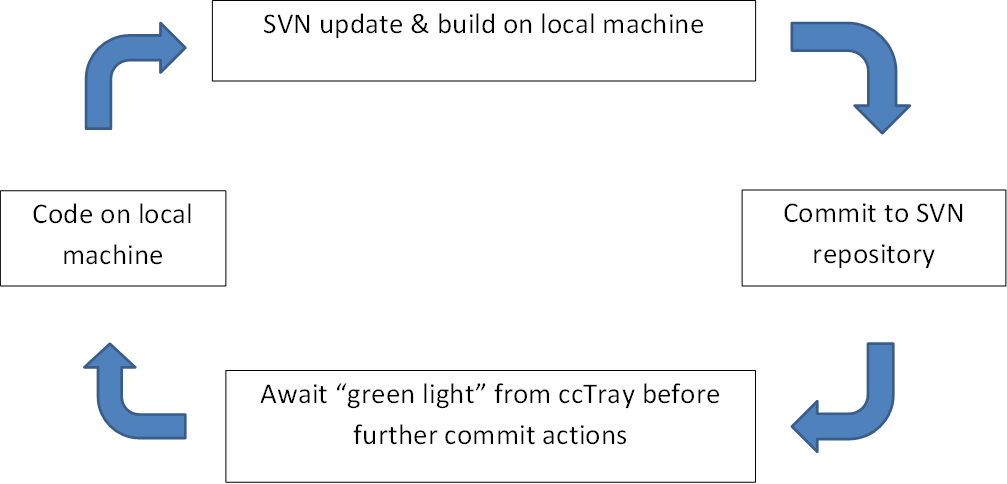
\includegraphics
			[scale=0.5]
			{images/ContinuousIntegration.png}
		\caption{The Continuous Integration Cycle}
		\label{fig:continuousIntegration}
	\end{center}
\end{figure}

A factor which was not taken into when considering \gls{ci} was the cost in time of setting up the software.  Further to this, the possibility of the server failing was not considered.  Naturally, the worst occurred during the project and the \gls{ci} software and all of its associated logs were lost.  The time spent on introducing \gls{ci} was not recouped in time saved by identifying problems and is not recommended for use in projects which feature only one developer, particularly if a low-risk hosting solution cannot be found.

\section{Bug Tracking}
\label{bugTracking}
Bug tracking is, as the name suggests, the tracing of the status of bugs that have been discovered in a system, used primarily to ensure that bugs which are found are dealt with or logged in a release.  It is another concept that was encountered while on summer industrial placement, and it struck the developer as an advantageous \gls{case} tool to utilise in this project.

The bug tracker was used when a bug was encountered that was not going to be fixed at the time of the discovery; the developer wanted to apply use of the bug tracker intelligently so that it was always going to be a help, and not a bureaucratic hindrance to development.  Bugs that were found were created in the system and given a priority, marked initially as `open' to symbolise that they had not yet been dealt with.  When a bug had been dealt with and the developer had verified that it was no longer an issue, it was marked as `closed', and remained in the system for traceability, should a similar issue crop up.  As a rule of thumb, a comment was recorded to say firstly what the problem was, secondly what the fix was and thirdly which \gls{svn} (see Section \ref{svn}) check-in fixed the issue so that one did not need to trawl through logs in \gls{svn} to find the fix, should they need to revisit it.

The software used was BugTracker.NET -- a free, open-source, web-based bug tracker.  Having encountered this particular product and worked with it for three months, the developer thought it wise to stick to familiar ground and employ the same product.  The developer used hardware running at home to deploy BugTracker.NET and used it until a server failure in late January 2011.  As the hardware was no longer reliable to host the software, the decision was taken to switch bug tracking software to SourceForge's Bug tracker, which worked in a similar way.  Bugs from the old system (both open and closed) were transferred to the new site and remain there now for traceability and reference.

The bug tracking software was highly useful during development of the product and ensured that discovered issues with the product were found and dealt with, or logged as known faults.  It is recommended to future projects to introduce a similar mechanism of defect tracking to ensure that problems do not go unresolved or are left forgotten.

\section{Acceptance Test}
For the project to pass the acceptance test, all unit tests associated with the project must be successful.  By the end of the project, there were approximately thirty unit tests, all of which passed.

This chapter has described the formal testing and bug management that took place on the product.  The next chapter assesses human evaluations on the project and establishes whether or not the usability aims of the project were realised.
\glsresetall{}
\chapter{Evaluation}
\label{eval}
This chapter discusses the evaluations that were carried out on the project.  In particular, it discusses the approaches that were taken, the results that were collected and the conclusions that can be drawn from the results, including future work for both the evaluations and the product.

It was necessary to perform evaluations with the assistance of people who were not directly involved with the project because an insider might not be able to provide a completely impartial examination of the system.

\section{General Approach}
The evaluation took two forms: firstly, a basic usability evaluation, focussing on a single user's interactions with the system; and secondly, an extended evaluation, examining the positive points and shortcomings of the system when multiple users were working with the system.

It was hoped that a sample of users external to the project, with various levels of knowledge of \bibtex and \LaTeX, would participate in the study.  Sampling a range of users was intended to ensure that the evaluation collected a representative spread of opinions on the product for analysis.

As the evaluation would involve other people, the `School of Computing Science Ethics Checklist'\footnote{The signed ethics checklist document is included as an appendix to this document.} was consulted to ensure that the intended evaluation was ethically sound and that it would not put participants at any greater risk than they encounter in their normal working lives.

The evaluations had slightly different environments and execution, which will be discussed within the relevant sections below.  The purpose of the two different evaluations are explained, and results are included with each of them.

\section{Basic Usability Evaluation}
The basic usability evaluation is based around the points raised in the background survey (Chapter \ref{backgrnd}).  Recall that the examination criteria in the background survey were centred around the \gls{ui} to the system, the features of the system and how fault tolerant and robust the system was.

\subsection{Environment}
The participant sat at a desk on an adjustable-height chair in a well-lit, quiet room at a comfortable temperature.	 Room 620 in the Boyd-Orr Building was the location for some of the experiments, others took place in the participant's office and some took place at the home of the developer.  The location and atmosphere of evaluations are mentioned to draw attention to the developer's conscious decision not to hold evaluations in an environment that was any more stressful, uncomfortable, abnormal or otherwise difficult than daily working conditions.

\subsection{Execution}
The following terminology is used consistently throughout this section: the `participant' means a volunteer who participated in an evaluation of the system and the `host' means the person who was running the evaluation; in all cases, the host was the developer of the system.

Evaluations were structured as follows:
\begin{enumerate}
	\item The host presented the participant with introduction script;\footnote{Introduction and debrief scripts are included as appendices to this document}
	\item The participant read the introduction script;
	\item The host asked the participant to verbally confirm that they agreed to take part in the evaluation;
	\item The participant agreed to take part;
	\item The participant was asked to familiarise themselves with the system by using the site for as long as they wished, and was encouraged to ask questions of the host;
	\item The participant told the host that they were ready to proceed;
	\item The host cleared the system and presented the participant with the task list\footnote{The task list is included as an appendix} and observed the participant, noting any points raised while performing tasks\footnote{The \gls{url} given to participants for import pointed to a search across the \gls{acm} library: \url{http://toms.acm.org/Volumes/V37.html?searchterm=bibtex}};
	\item The participant told the host that they had completed the task list;
	\item The host gave the participant a questionnaire, which they filled in. Notes taken by the host on the participant's behalf were given to them to remind them of things they had mentioned;
	\item The participant gave the host the completed questionnaire, which was put into an opaque folder in a random order, to help preserve participants' anonymity;
	\item The host gave the participant the debrief script;
	\item The participant took a note of the email addresses provided and was given a final chance to ask questions during the evaluation;
	\item The host thanked the participant for their time.
\end{enumerate}

While the participant was performing tasks, the host noted relevant points that the participant raised.  This was done in an attempt to help the participant to focus on the task at hand, rather than leaving the participant to recall the comments they made; it also allowed the host to gain a better insight into any difficulties encountered by the participant.

\subsection{Results}
Tabulate results from the evaluations and go on to analyse the results.

\subsection{Analysis}
Sample of users - some CS students targeted, Physics/Astronomy students, staff and users who don't have academic knowledge - relevant point? why use them? Worth mentioning at all?

\subsection{Improvements Made}

\section{Extended Usability Evaluation}
The second type of usability evaluation was aimed at testing the multi-user functions of the system, in particular the effectiveness of the system to keep users up to date with what has happened. 

\subsection{Environment}
A single session was held in room 620 of the Boyd-Orr Building, under the same conditions as the basic evaluation previous to it.

\subsection{Execution}
The execution involved participants

\subsection{Results}
\subsection{Analysis}

\subsection{Improvements Made}

\section{Summary of Evaluations}

\subsection{Potential Improvements to Evaluations}

\glsresetall{}
\chapter{Conclusion}
\label{conclusion}
The conclusion chapter of this dissertation draws to a close the discussion of the project.

It performs a retrospective assessment of the successes and shortcomings of the project with respect to the aims and identifies some future work for the area.

Finally, it analyses the personal development that the author went through during the project and some of the lessons learned about single-developer projects.

\section{Summary}
Upon reflection on the aims of the project, the author feels that the final year undertaking was a success.

It is felt that a far better understanding of the technologies used has been gained, particularly in the areas of NHibernate and \gls{asp}\gls{net}.  

It is also felt that good software engineering practice during development and testing was undertaken.  With that said, it was realised during development of the system that some of the practice employed turned out to be more of a bureaucratic and unnecessary measure than an assistive process.  Common sense prevailed in these scenarios, and were particularly noticeable by the scaling back of unit testing and \gls{ci}.  

Some software engineering practices were helpful.  The bug tracking software was especially helpful having been employed with a common-sense approach in mind.  Its greatest benefit was that it ensured that defects with the software did not go unnoticed or unresolved.

The professional attitude that has been developed by the author over approximately six months has been career-changing for the better.  The project required deep knowledge and understanding at every stage of the project.  The author had to perpetually be on top form; had he not been, he would not have been exposed to as many important concepts, would not have learned as much and would not have produced as usable or useful a system as was done.

The software solution produced was found to be a success --- an outcome determined by statistical analysis of evaluation participants� responses to a questionnaire. The measurements derived from this showed that all participants reacted positively to questions on the usability of the software solution Moreover, they encouraged further development of the solution and even suggested specific areas of further work.

It might work in the developer's favour to alert the reader to the fact that the bibliography for this dissertation was managed entirely by the software product produced this year.  

\section{Suggestions for Further Work}
Suggestions of areas for further work on this software solution include:
\begin{enumerate}
	\item Allow the tagging of entries (as set out in the Discovery model); 
	\item Implement a help system for users;
	\item Allow users to upload to a tag;
	\item Allow users to download a tag or specific set of entries;
	\item Allow the grouping of users with privileges attached to their roles;
	\item Use a push-based approach for concurrent access rather than polling the server.  Many redundant packets are sent and received because of the approach taken at the moment.  It would be better in terms of performance, server load and scalability if the system did not have to frequently respond with empty replies;
	\item Use a more rigorous approach to authentication.
\end{enumerate}

\section{Personal Lessons and Professional Development}
The author of this dissertation underwent substantial personal development during the production of this software solution, particularly in terms of technical knowledge gained, professional conduct and software engineering discipline gained.

It was also reassuring to confirm that the author's choice of software engineering as a career is an absolutely suitable and exciting path, having thoroughly enjoyed the challenge of working with Dr Manlove to design, produce, evaluate and discuss the software solution offered by the project.


\appendix

\printglossaries

\bibliographystyle{plain}
\bibliography{l4proj}
\end{document}
